 % Outline:
% \begin{enumerate}
% \item What are evaluation functions?
% \item Traditional definition of $k$-ply search
% \item Modified $k$-ply search for HackAttack
% \end{enumerate}

% what is a strategy, and evaluation function?
A strategy for a game is a function that takes as input a player's situation and returns that player's move(s). There are many ways to develop strategies. A common approach in the cyber security game theory literature is to explicitly write down the objective function and then directly derive optimal solutions. This approach works well only in the simplest games, such as static matrix games. For more complex games, such as stochastic Markov games, alternative methods (e.g., Q-Learning) can be used~\cite{alpcan2006intrusion}. However, the most complex games must adopt methods similar to those used to develop strategies for checkers and chess. These approaches involve the development and use of {\em evaluation functions} to score the desirability of any possible state of the game. The evaluation function is a formalization of expert intuition on what constitutes a good position. For example, in the game of chess, it may include points for material, controlling the center of the board, having freedom to move, and so on. The evaluation function is then used in a multiple look-ahead tree search to select the best move to play.

% example evaluation function
As a simple example, a possible tic-tac-toe evaluation function is described in Figure~\ref{fig:tictactoe}. Such an evaluation function can then be used to consider what-if scenarios and select a move. For example, Figure~\ref{fig:tictactoe} shows a board and two possible moves that have been scored according to this evaluation function. This approach suggests that the second move is preferable to the first. 

\begin{figure}[h!tbp]
\begin{center}
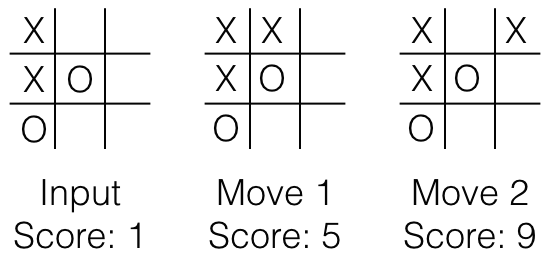
\includegraphics[width=2.8in]{ttt.png}
\caption{An evaluation function for scoring the tic-tac-toe board for player X could be defined by granting 4 points for each open two-in-a-row that X has, subtracting 1 for each one O has, subtracting 1 point if O occupies the center, and adding 3 points for each corner occupied by X.
According to this evaluation function, X would prefer Move 2 to Move 1 since it has a higher score.\label{fig:tictactoe}}
\end{center}
\end{figure}

In practice, however, it can be very difficult to engineer an evaluation function that fully captures the intricacies of the game. The value of a game state depends on the possible responses by the opponents. 
For example, points could be added if a good move could be possible on the next turn and subtracted if the opponent can make a good move. 
The combinatorial possibilities make such an evaluation function difficult to define and harder to tune.
Rather than attempt to construct a highly complex evaluation function, an alternative method is to ``look several moves ahead'' by searching a tree of subsequent possible.

\begin{figure}[h!tbp]
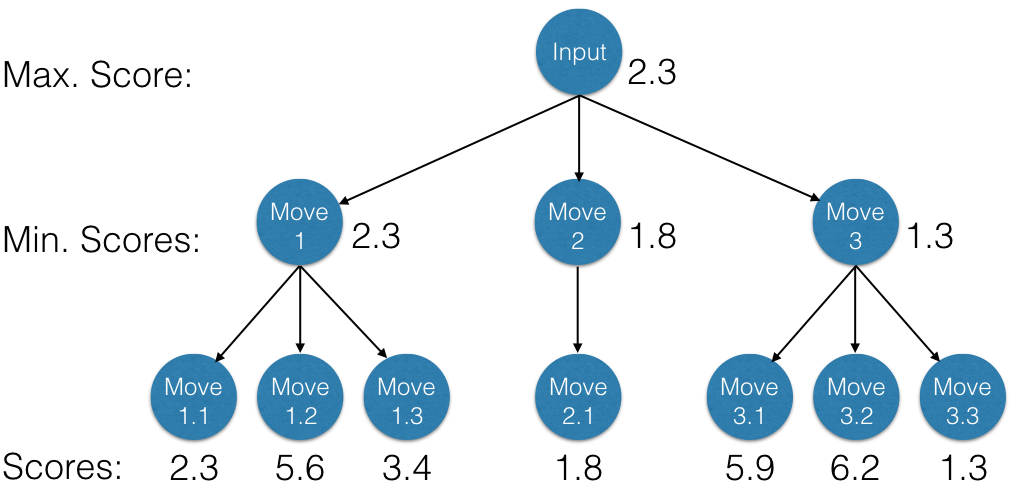
\includegraphics[width=3.3in]{tree-pic2.png}
\caption{A 2-ply tree search explores all moves, starting from an input state, to create the middle layer of the tree. From each of those states, all possible opponent moves are considered. The leaf nodes are then scored by the evaluation function. The middle layers are assigned a score, not from the evaluation function applied to their states, but as the minimum of their children's scores. The root node is given the maximum of its children's scores. In this case the best move would be Move 1, since it was the source of the high score.\label{fig:minmaxtree}}
\end{figure}

As shown in Figure~\ref{fig:minmaxtree}, a tree is constructed top-down starting with the current board configuration as the root. For each possible move, a child node is created. This makes up the {\em 1-ply} tree. Then, at each leaf, each opponent move is added as a child, making up the {\em 2-ply} tree. This process continues to the desired depth. At the bottom, each board configuration is scored according to the evaluation function. These scores are then rolled up as follows. If the last move represents the player's move then, under the assumption that the player will try to improve the board, the maximum of the childs' scores are assigned to the parent. On the other hand, if the last move represents the opponent's move then the minimum is used. This process is repeated up the tree, alternating between min and max. The score given to the root is the largest value among its children (which may occur multiple times). One of these highest-scoring moves is then selected. This is the {\em $k$-ply strategy} for the given evaluation function. Evaluation functions and $k$-ply search trees have been used to analyze a wide variety of games~\cite{levy2009computer}. 

The basic $k$-ply strategy assumes that all possible moves are known and deterministic. It also assumes that each player gets one move. In HackAttack, results are probabilistic and the number of moves a player gets next turn depends on the outcome of their move this turn. Furthermore, each player has only limited knowledge of the other players' knowledge, accounts, and exploits. This lack of knowledge makes it very difficult to consider the opponent's best move; that would require the computationally intractable problem of branching over all possible assets the opponent may have and averaging the results according to the probabilities. Consequently, we adopted some simplifying assumptions and explored two different kinds of $k$-ply search: Random-Response and No-Response.

% Random-Response: your move and then random move
In a Random-Response $k$-ply search, the opponent's move is modeled as being randomly chosen from all possible moves. The probability of each move is weighed by the probability that the opponent would have the resources to carry out the move, according to the player's knowledge. To this end, each player's knowledge of the other player had to be tracked, which is described below.

% No-Response: only think about your own moves
In a No-Response $k$-ply search, the opponent moves are not considered. Each level of the tree contains the next possible moves for the player. This approach has the disadvantage of not being able to account for enemy choices. However, in HackAttack, often very little is known about the enemy and their resources, which makes it difficult to respond meaningfully. In this tree search, each node is assigned the maximum score of its children nodes. The main advantage of the No-Response $k$-ply search is that it is possible to develop more elaborate (i.e., multi-step) plans.
The name No-Response indicates that it plans ahead as if no response will be brought against its actions, but the strategy itself can still respond to its opponent. 
For example, if a successful {\tt hack} is detected, it could decide to {\tt clean} that computer in response.
 
% simplifying assumption: only consider one resource's move at a time, then think about the outcome of that as the starting point for the next resource
In HackAttack, a player is allowed one move for each computer on which they have at least one account. This means that a player with, say, 5 accounts, would have an enormous number of possible moves. This combinatorial explosion slows the tree search and makes it impractical for analysis. To avoid this issue, we consider a single computer at a time. A tree is created for the moves from that computer, and the best move is chosen. The result of that move is then used as the starting point of a tree search for the next computer. This approach is less thorough and may miss some possibilities for coordinating actions, but it turns a multiplicative work factor into an additive one. 

% knowledge tracking
The information at each node in the search tree is a knowledge structure. It contains four tables of probabilities indicating the player's degree of belief in various claims. 
The probabilities are updated using Bayes's Theorem when the player observes something (e.g., the result of their action or the detection of an opponent's action).
The first table gives the probability of each host having a particular OS. The second table tracks the probability of each machine being patched against each exploit. The third table provides the probability of player $p$ having $r$ accounts on computer $c$. The last table contains the probability that player $p$ has each possible exploit. 

The use of a $k$-ply tree search requires the specification of an evaluation function. For the purposes of this research, we used a ``net-computers'' evaluation function, which is the number of computers the player has accounts on minus the expected (in the probabilistic sense) number of computers the opponent has. (The expected number is used because the exact number is not known to the players.) 
